
\chapter{Non-Linear Functions}\label{Chapter:NonLinear}


\section{Quadratic Functions}\label{Section:Quadratics}



\subsection{Form of Quadratic functions}

\begin{definition}
A function $q(x)$ is a \textbf{ quadratic function} if it may be written as: $$q(x)=ax^2+bx+c.$$ where $a\neq0$.
\end{definition}

The classic example is the standard parabola,  $y=x^2$ or a quadratic with $a=1. b,c=0$.  \url{https://www.desmos.com/calculator/aktz8g8cbh}.  We should be familiar with some of the properties of this shape, it's symmetric on both sides and it goes to positive  infinity in both directions (as $x^2$ cannot be negative).\\

It would be nice if we could show that all quadratics had the same essential shape.  To do this, we must first show that all quadratics also have the form $$q(x)=a(x-h)^2+k.$$

To see this:

\begin{eqnarray*}
q(x)&=&ax^2+bx+c\\
&=&a(x^2+\frac{b}{a}x)+c\\
&=&a(x^2+2\frac{b}{2a}x+\frac{b^2}{4a^2})+c-\frac{b^2}{4a}\\
&=&a(x+\frac{b}{2a})^2+c-\frac{b^2}{4a}\\
\end{eqnarray*}
So by letting $h=-\frac{b}{2a}$ and $k=c-\frac{b^2}{4a}$, we have our form.\\

An interesting byproduct of this is that if we were to solve $ax^2+bx+c=0$, we would get:

\begin{eqnarray*}
ax^2+bx+c&=&0\\
a(x+\frac{b}{2a})^2+c-\frac{b^2}{4a}&=&0\\
a(x+\frac{b}{2a})^2=\frac{b^2}{4a}-c\\
a(x+\frac{b}{2a})^2=\frac{b^2-4ac}{4a}\\
(x+\frac{b}{2a})^2=\frac{b^2-4ac}{4a^2}\\
x+\frac{b}{2a}=\frac{\pm\sqrt{b^2-4ac}}{2a}\\
x=\frac{-b\pm\sqrt{b^2-4ac}}{2a}\\
\end{eqnarray*}

Which is the quadratic formula.

\subsection{Parabolas}

Now that we have this form $a(x-h)^2+k$, consider how $a,h,$ and $k$  affect the shape of the graph: \url{https://www.desmos.com/calculator/4zqd9chlna}.\\

Sliding $k$ shifts the parabola up and down.  We can think of this as adding to or detracting from the value of $x^2$.  Sliding $h$ shifts the graph left and right.  We can think of this as slowing down or speeding up $x^2$ by $h$ units.  $a$ stretches or squashes $x^2$, or if $a$ is negative, also reflects this across the $x$ axis.  But all of these transformations preserve the fundamental shape of a parabola, so all quadratic functions have this shape.



\section{Polynomials}\label{Section:Polynomials}


\begin{definition}

A \textit{polynomial} $p(x)$ is a function that can be written in the form $$p(x)=a_nx^n+a_{n-1}x^{n-1}+\cdots+a_1x^1+a_0(x^0),$$ where $n\geq 0$ is a whole number, and $a_n\neq 0$ \textbf{unless} $p(x)=0$.

\begin{itemize}
\item The $a_i$ are the \textit{coefficients} of $p(x)$.
\item $a_n$ is the \textit{leading coefficient} of $p(x)$.
\item $n$ is the \textit{degree} of $p(x)$.
\item $a_nx^n$ is the \textit{leading term}  of $p(x)$.
\end{itemize}


\end{definition}

\subsection{Long Term Behavior}

When we consider a polynomial $p(x)=a_nx^n+a_{n-1}x^{n-1}+\cdots+a_1x^1+a_0$, we notice that no matter how big the coefficients $a_{n-1}$ through $a_0$ are, they will all eventually be made insignificant by $x^n$ for some sufficiently large values of $x$.  Thus we have the following fact:

\begin{remark}
The long term behavior of $p(x)$ is determined \textbf{completely} by it's leading term $a_nx^n$.
\end{remark}

So we have 2 things to consider, whether or not $a_n$ is positive or negative, or whether or not $n$ is even or odd. \\

If $a_n>0$, then there are 2 possibilities:

\begin{itemize}
\item If $n$ is even, (like $x^2, x^4, x^6)$, then $a_nx^n$ cannot be negative, so $p(x)$ will tend to positive infinity as $x$ goes to either positive or negative infinity.
\item If $n$ is odd, (like $x, x^3, x^5)$, then $a_nx^n$ is positive as long as $x$ is positive, so $p(x)$ will tend to positive infinity as $x$ goes to either positive infinity, and $a_nx^n$ will go to negative infinity as x goes to negative infinity.
\end{itemize}
Then, if $a_n<0$, everything is flipped upside down.  We can summarize as follows:
$$
\begin{tabular}{c|c|c|}
 & $n$ even & $n$ odd\\
\hline 
$a_n>0$ & $p(x)\to \infty$ as $x\to \infty, -\infty$& $p(x)\to  \begin{cases}\infty & x\to \infty\\ -\infty & x\to -\infty \end{cases}$\\
\hline 
$a_n>0$ & $p(x)\to -\infty$ as $x\to \infty, -\infty$& $p(x)\to  \begin{cases}-\infty & x\to \infty\\ \infty & x\to -\infty \end{cases}$\\
\hline
\end{tabular}
$$
\subsection{Short Term Behavior}
The first thing one can always do when analyzing the short term behavior of $p(x)$ is find the $y$-intercept.  The $y$ intercept is just the point on the curve of the function when $x=0$, so this is $p(0)=a_0$.\\

By the \textbf{Fundamental Theorem of Algebra}, we can write $p(x)=a_nx^n+\cdots +a_0$ as: $$p(x)=a_n(x-r_1)^{m_1}(x-r_2)^{m_2}\cdots (x-r_k)^{m_k}\cdot q_1(x)q_2(x)\cdots q_\ell(x)$$
where the $q_i(x)$ are irreducible quadratics.  We call $r_1, \ldots, r_k$ the \textit{roots} of $r(x)$, where root $r_i$ has \textit{multiplicty} $m_i$.  What this means is if we plug $r_i$ into $p(x)$, we end up with 0, since that linear factor ends up being 0.\\

The behavior of $p(x)$ around these roots is determined by the multiplicity of that root.  We know that $p(x)$ will be 0 at those roots, so the question is whether or not the polynomial crosses the $x$ axis at a given roots, or bounces off the axis:

$$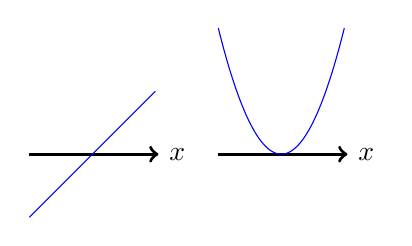
\begin{tikzpicture}[scale=.4][domain=-2:2]
%    \draw[gray!50, thin, step=1] (-10,-5) grid (11,5);
    \draw[very thick,->] (-2,0) -- (2.1,0) node[right] {$x$};
%    \draw[very thick,->] (0,-5) -- (0,5.1) node[above] {$y$};

%    \foreach \x in {-10,...,10} \draw (\x,0.05) -- (\x,-0.05) node[below] {\tiny\x};
%    \foreach \y in {-4,...,4} \draw (-0.05,\y) -- (0.05,\y) node[right] {\tiny\y};


  \draw[scale=1,domain=-2:2,smooth,variable=\x,blue] plot ({\x},{\x});% node[above]{$f(x)$};

    \draw[very thick,->] (4,0) -- (8.1,0) node[right] {$x$};
%    \draw[very thick,->] (0,-5) -- (0,5.1) node[above] {$y$};

%    \foreach \x in {-10,...,10} \draw (\x,0.05) -- (\x,-0.05) node[below] {\tiny\x};
%    \foreach \y in {-4,...,4} \draw (-0.05,\y) -- (0.05,\y) node[right] {\tiny\y};


  \draw[scale=1,domain=4:8,smooth,variable=\x,blue] plot ({\x},{(\x-6)^2});% node[above]{$f(x)$};



\end{tikzpicture}$$ % of mbox

We notice that $p(x)$ only changes sign when it's factors $(x-r_i)^{m_i}$ changes sign.  But $(x-r_i)^{m_i}$ only changes sign if $m_i$ is odd.  So we have the following fact:
\begin{remark}
The polynomial $p(x)$ ``crosses" the $x$-axis at $r_i$ if $m_i$ is odd and ``bounces" if $m_i$ is even.
\end{remark}

\begin{example}
Let $$p(x)=x^3-3x^2=x^2(x-3).$$  \url{https://www.desmos.com/calculator/iy0chaljdq} Since it is a odd degree polynomial with positive leading coefficient, it goes up to $\infty$ as $x$ goes to $\infty$ and down to $-\infty$ as $x$ goes to $-\infty$.  We also see that $p(x)=0$ whenever $x=0$ or $x=3$.  The multiplicity of 0 is 2, and the multiplicity of 3 is 1, which are even and odd respectively, so $p(x)$ ``bounces" at $x=0$ and crosses at $x=1$.

$$  \begin{tikzpicture}[scale=.5]
    \begin{axis}[
        restrict y to domain=-5:5,
        samples=1000,
        minor tick num=1,
        xmin = -3, xmax = 4,
        ymin = -5, ymax = 5,
        unbounded coords=jump,
        axis x line=middle,
        axis y line=middle]

      \addplot[mark=none, domain=-3:4] {\x^3-3*\x^2};
    \end{axis}
  \end{tikzpicture}$$
 % of mbox



\end{example}



\begin{example}
Let $$p(x)=x^4-2x^2+1=(x-1)^2(x+1)^2.$$  \url{https://www.desmos.com/calculator/wmr67oopgj}  Since it is a even degree polynomial with positive leading coefficient, it goes up to $\infty$ as $x$ goes to both positive and negative $\infty$.  We also see that $p(x)=0$ whenever $x=-1$ or $x=1$.  The multiplicity of both of these roots is 2,  so $p(x)$ ``bounces" at both $x=1$ and $x=-1$.

$$  \begin{tikzpicture}[scale=.5]
    \begin{axis}[
        restrict y to domain=-5:5,
        samples=1000,
        minor tick num=1,
        xmin = -3, xmax = 3,
        ymin = -5, ymax = 5,
        unbounded coords=jump,
        axis x line=middle,
        axis y line=middle]

      \addplot[mark=none, domain=-3:3] {\x^4-2*\x^2+1};
    \end{axis}
  \end{tikzpicture}$$
 % of mbox



\end{example}









\section{Rational Functions}\label{Section:RationalFunctions}

\begin{definition}
A \textbf{rational function} is a function $r(x)$ which may be written as $r(x)=\frac{p(x)}{q(x)}$ where $p(x), q(x)$ are both polynomials, and $q(x)\neq 0$.
\end{definition}

Now when we say $q(x)\neq0$, we mean that $q(x)$ is not the polynomial 0, not that $q(x)$ could never be 0.  As before, we will consider the long and short term behavior of polynomials.

\subsection{Long Term Behavior}

For Polynomials, what determined the long term behavior of a polynomial was the leading term.  So it makes sense that a rational function will be determined the same way.  Given  $$r(x)=\frac{a_nx^n+\cdots a_0x^0}{b_mx^m+\cdots b_0x^0},$$ we can determine the long term behavior with $$\frac{a_nx^n}{b_mx^m}$$ which simplifies to $\frac{a_n}{b_m}x^{n-m}$.  So there are some cases to consider here:

\begin{itemize}
\item If $n>m$, then $\frac{a_n}{b_m}x^{n-m}$ is just a regular monomial.  This doesn't mean that $r(x)$'s graph will look like a polynomial's, but it does mean the long term behavior will be the same as that of a polynomial.\\

For example consider $y=\frac{-x^4+x}{x+1}$.  We should note: $\frac{-x^4-x}{x+1}\sim\frac{-x^4}{x}
\sim -x^3$, so the long term behavior of $y$ will be the same as $-x^3$'s:  positive infinity to the left, negative infinity to the right.  \url{https://www.desmos.com/calculator/jzxyyrcgep}.

\item If $n=m$, then $\frac{a_n}{b_m}x^{n-m}=\frac{a_n}{b_m}$ is just a constant.  So as the magnitude of $x$ grows, these values approach $\frac{a_n}{b_m}$.\\

For example consider $y=\frac{-2x^4+x}{3x^4+1}$.  We should note: $\frac{-2x^4-x}{3x^4+1}\sim\frac{-2x^4}{3x^4}
\sim -\frac{2}{3}$, so the long term behavior of $y$ will be the same as $-\frac{2}{3}$'s:   \url{https://www.desmos.com/calculator/qaeq86mivp}.
 
\item If $n<m$, then $\frac{a_n}{b_m}x^{n-m}=\frac{a_n}{b_m}\frac{1}{x^{m-n}}$.  As the magnitude of $x$ grows, the more $\frac{1}{x^{m-n}}$ will shrink and the entire function converges to 0.\\

For example consider $y=\frac{-2x^2+x}{3x^4+1}$.  We should note: $\frac{-2x^2-x}{3x^4+1}\sim\frac{-2x^2}{3x^4}
\sim -\frac{2}{3}\frac{1}{x^2}$, so the long term behavior of $y$ will be converging to 0:   \url{https://www.desmos.com/calculator/n0ftbxmcod}.
 
 
\end{itemize}


\subsection{Short term behavior}

Here, we once again care about the multiplicity of the roots, that is, if $r(x)=\frac{p(x)}{q(x)}$, what we care about is when $p(x)$ or $q(x)$ is 0, and what the multiplicity is.\\

Well, turns out, 0 divided by anything is 0.  So if the numerator is 0, then $r(x)$ is 0.  Moreover, it bounces or crosses in the same way as a polynomial.  So if the multiplicity is odd, the function crosses and if it's even, it bounces.\\

For example, consider $r_1(x)=\frac{x-1}{x}$.  It is clearly 0 when $x=1$, and since the multiplicity is odd, we cross \url{https://www.desmos.com/calculator/9graa40kq1}.  But if we change that to $r_2(x)=\frac{(x-1)^2}{x}$, the multiplicity is now even so we bounce \url{https://www.desmos.com/calculator/iy9kvoac37}.\\

It also turns out you can't divide by 0.  So at those points, the function is undefined.  And as the values in the denominator towards 0, the overall value of the quotient approaches either positive or negative infinity.  Just like roots, whether or not we change signs at these asymptotes depends on the multiplicity of the root.\\




For example, again consider $r_1(x)=\frac{x-1}{x}$.  The denominator is 0 when $x=0$, so we have a vertical asymptote there.  Since the multiplicity is odd, we change signs there: \url{https://www.desmos.com/calculator/ik9xwhui5i}.  If we made that multiplicity even, the function would not change sign at $x=0$, so for $r_2(x)=\frac{x-1}{x^2}$: \url{https://www.desmos.com/calculator/h5famtu30t}






\section{Exponentials}\label{Section:Exponentials}

\begin{definition}
An \textbf{exponential function} is a function $f(x)$ which may be written as $f(x)=b\cdot a^x$.
\end{definition}

We should note that we've seen exponential functions before, in the guise of compound interest.  If the future value of a debt is $S=P(1+i)^x$ after $x$ unites of time, then $P$ is your $b$ and $1+i$ is your $a$.\\

We should also note that there is a real kinship between exponential functions and linear functions.  Linear functions have the form $\ell(x)=mx+b$, which we can think of as $\ell(x)=\overbrace{m+m+\cdots+m}^x+b$, with $x$ copies of $m$.  Similarly we can see that $f(x)=b\cdot a^x=\overbrace{a\cdot a\cdots a}^x\cdot b$, so it is really the multiplicative analogue of the linear function, where the $b$'s are the initial value of the function when $x=0$ and the growth rate of the function is totally determined by $a$ (whereas it's determined by $m$ for linear functions).\\

In that way, we can also tell when $f(x)=b\cdot a^x$ is increasing or decreasing, just by looking at whether or not $a>1$ or $a<1$.  If $a>1$ it is increasing: \url{https://www.desmos.com/calculator/edktzphc6x} if $a<1$ then it's decreasing: \url{https://www.desmos.com/calculator/rpiu9qc4ty}.\\


Exponential functions are used to model anything that grows or decays proportionately to  it's current value.  So for example debts or investment accrue proportionately to how much debt/investment there already is.  Population is another example, the greater the population, the more reproduction there will be within that population and the greater the increase in population.

\section{Logarithms}\label{Section:Logarithms}

So looking at any exponential function, but specifically for increasing ones, we notice that they are 1-1, meaning two different inputs give you 2 different outputs.  Thus, $f(x)=a^x$ is an invertible function.  You can see in these graphs \url{https://www.desmos.com/calculator/cvriy608bg} that reflecting the exponential over the $y=x$ line giving us the green function is another function.  We call this function $\log_a(x)$.  As the inverse of an exponential function, it has some properties:

\begin{itemize}
\item \textbf{It's domain is only positive numbers}.  Why?  Because the only possible outputs of exponential outputs are positive numbers.  Taking the inverse reverses the roles of the domain and range, and so the domain of $\log_a$ is the positives.
\item \textbf{As $\mathbf{x}$ goes to 0, $ \mathbf{\log_a(x)}$ goes to $\mathbf{-\infty}$.}   This is the result of the reflection.  Normally $a^x$ (for $a>1$) goes to 0 as $x\to -\infty$, so when reflected, that line is now asymptotic to the $y$-axis.  Also $\log_a$ returns the power necessary to achieve the value $x$.  If $x$ is a small number like 0.0001, what power would I have to raise $a$ to to get $0.0001$?  It can't be 0, $a^0=1$, so it has to be \textbf{less} than 0, and the smaller $x$ is, the lower this power must go.

\item  As $\mathbf{x\to\infty, \log_a(x)\to \infty}$, again this is the result  of the reflection, but we can also think of this as the powers $a$ needs to be raised to in order to achieve $x$, as this increases, those powers must increase as well.

\item $\log_a(xy)=\log_a(x)+\log_a(y)$. Too see this consider:

\begin{eqnarray*}
xy&=&a^{\log_a{xy}}\\
xy&=&x\cdot y\\
&=&a^{\log_a(x)}\cdot a^{\log_a(y)}\\
&=&a^{\log_a(x)+\log_a(y)}.
\end{eqnarray*}


\item $\log_a(x^y)=y\log_a(x)$.  To see this, consider:

\begin{eqnarray*}
x^y&=&a^{\log_a(x^y)}.\\
x^y&=&(a^{\log_a(x)})^y\\
&=&a^{y\log_a(x)}
\end{eqnarray*}



\end{itemize}

Typically most textbooks include a whole bunch of other arithmetic rules, but they can all be distilled from the 2 above so they're all totally pointless.\\

Special cases of logs are log base 10 which is usually just denoted $\log$ and log based $e$, which is denoted $\ln$.  Astronomers and other scientists like $\log$ since taking $\log$ base 10 gives you approximate magnitude of stuff.  As a mathematician, I prefer $\ln$ since $e$ has pretty special mathematical properties, plus it's shorter, which makes it better.\\

The main use of logs algebraically is to de-exponentiate expressions.  So if one is trying to solve $10=2^x$, we could do this via:

\begin{eqnarray*}
10&=&2^x\\
\ln(10)&=&\ln(2^x)\\
\ln(10)&=&x\ln(2)\\
x&=&\frac{\ln(10)}{\ln(2)}\approx 3.3219.
\end{eqnarray*}

One can also solve problems like this visually:  \url{https://www.desmos.com/calculator/t0pojr0gel}.












